\documentclass[a4paper,10pt,article]{memoir}
\usepackage[utf8]{inputenc}
\usepackage[danish]{babel}
\usepackage{graphicx}
% Hyppigt benyttede pakker

\usepackage{amsmath}
\usepackage{amssymb}
\usepackage{amsthm}
\usepackage{listings}
\usepackage{color}

% Farver

\definecolor{dkblue}{rgb}{0,0.1,0.5}
\definecolor{dkgreen}{rgb}{0,0.4,0}
\def\Red{\color{\ifdraft red\else black\fi}}
\def\Green{\color{\ifdraft green\else black\fi}}
\def\Blue{\color{\ifdraft blue\else black\fi}}
\def\Black{\color{black}}
\newcommand{\details}[1]{\iffull{\Blue#1}\fi}
\definecolor{linkColor}{rgb}{0,0,0.5}

% S�tninger mv.

\newtheorem{theorem}{Theorem}
\newtheorem{corollary}[theorem]{Corollary}
\newtheorem{lemma}[theorem]{Lemma}

\newtheorem{saetning}{S{\ae}tning}
\newtheorem{proposition}{Proposition}
\newtheorem{korollar}{Korollar}

\theoremstyle{definition}
\newtheorem{definition}{Definition}
\newtheorem{example}{Example}
\newtheorem{eksempel}{Eksempel}
\newtheorem{problem}[theorem]{Problem}

\newenvironment{bevis}{\begin{proof}[Bevis:]}{\end{proof}}

% Operationel semantik

\newcommand{\lag}{\langle}
\newcommand{\rag}{\rangle}
\newcommand{\setof}[2]{\ensuremath{\{ #1 \mid #2 \}}}
\newcommand{\set}[1]{\ensuremath{\{ #1 \}}}
\newcommand{\besk}[1]{\ensuremath{\lag #1 \rag}}
\newcommand{\ra}{\rightarrow}
\newcommand{\lra}{\longrightarrow}
\newcommand{\Ra}{\Rightarrow}

% M�ngdenotation

\newcommand{\pow}[1]{\mathcal{P}(#1)}
\newcommand{\Z}{\ensuremath{\mathbb{Z}}}
\newcommand{\Nat}{{\mathbb N}}
\newcommand{\Binary}{{\mathcal B}}
\newcommand{\defeq}{\stackrel{\mathrm{def}}{=}}

\newcommand{\dom}[1]{\mbox{dom}(#1)}
\newcommand{\ran}[1]{\mbox{ran}(#1)}

% Udsagnslogik

\newcommand{\logand}{\wedge}
\newcommand{\logor}{\vee}
\newcommand{\True}{\mathbf{t \! t}}

% Parenteser

\newcommand\lb {[\![}
\newcommand\rb{]\!]}
\newcommand{\sem}[1]{\lb #1 \rb}
\newcommand{\subst}[2]{\{  {}^{#1} / {}_{#1} \}}

\newenvironment{tuborg}{\left\{ \begin{array}{cc} }{\end{array} \right.}

% Flexible-length arrows (Copyright (C) 1995, Michael Rettelbach)

\makeatletter
\newdimen\lleng
\newdimen\bleng

\def\gummitrans#1{
  \setbox0=\hbox{$\stackrel{\,#1}{\mbox{}}$}
  \lleng=\wd0%
  \advance\lleng by 0.6em
  \;\raisebox{0ex}{$\stackrel{\,#1}{%
    \makebox[\lleng]{%
      \rule{0mm}{1ex}\mbox{}\leavevmode \xleaders
      \hbox {$\m@th \mkern -2.6mu \relbar \mkern -2.6mu$}\hfill\mbox{}}}$}%
  \hspace{-2.2ex}\rightarrow}

\def\Gummitrans#1{
  \setbox0=\hbox{$\stackrel{\,#1}{\mbox{}}$}
  \lleng=\wd0%
  \advance\lleng by 0.6em
  \;\raisebox{0ex}{$\stackrel{\,#1}{%
    \makebox[\lleng]{%
      \mbox{}\leavevmode \xleaders
      \hbox {$\m@th \mkern -2.6mu \Relbar \mkern -2.6mu$}\hfill\mbox{}}}$}%
  \hspace{-2.2ex}\Rightarrow}

\def\trans#1{\mathrel{\gummitrans{#1}}}
\def\Trans#1{\mathrel{\Gummitrans{#1}}}


% Bevisregler

% Med sidebetingelse

\newcommand{\condinfrule}[3]
           {\parbox{5.5cm}{$$ {\frac{#1}{#2}}{\qquad
            #3} \hfill  $$}}

% Uden sidebetingelse

\newcommand{\infrule}[2]
           {\parbox{4.5cm}{$$ \frac{#1}{#2}\hspace{.5cm}$$}}

% Regelnavn

\newcommand{\runa}[1]{\mbox{\textsc{(#1})}}

% Svar p� sp�rgsm�l

\newenvironment{svar}{\begin{quote}\noindent\textbf{Svar:}}{\end{quote}}


\title{Tavlenoter \\ \emph{Nondeterministiske endelige automater}}
\author{Mette Thomsen Pedersen}
\date{7. februar 2013}

%%% BEGIN DOCUMENT
\begin{document}
\maketitle

\tableofcontents*

\chapter{Indledning}

Denne forelæsning handler om

\begin{itemize}
\item Definition af NFA'er.
\item Accept.
\item NFA'er og DFA'er er ækvivalente. - Enhver NFA N kan konverteres til en DFA M.
\item De regulære sprog er lukket under U, $\circ$ og $\ast$.

\end{itemize}

\chapter{Definition af NFA'er.}
\section*{Eksempel}

Lad $L_1$ være et sprog. Så er
\[ L_1 = \setof{w \in \set{0,1}^{\ast}}{ w \text{ indeholder et lige antal 0'er eller have præcis to forekomster af 1} }\]
%
Et eksempel på hvad sproget accepterer kan ses herunder:

\[ 0011 \in L_1, 000111 \notin L_1 \]
Lad så

\begin{align*}
L_1 & = L_1' \cup L_1'' \\
L_1' & = \setof{w \in \set{0,1}^{\ast}}{ w \text{ har et lige antal 0'er}}
L_1'' = \setof{w \in \set{0,1}^{\ast}}{ w \text{ har præcis to 1'ere}}
\end{align*}

\begin{figure}[h]
\centering
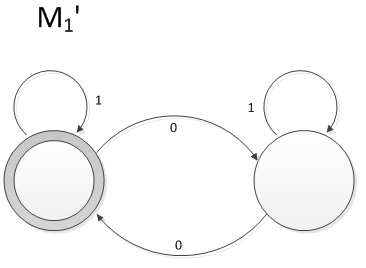
\includegraphics[scale=0.8]{figur1.png}
\caption{$M'_1$ er en DFA.}
\label{fig:1}
\end{figure}

\begin{figure}[h]
\centering
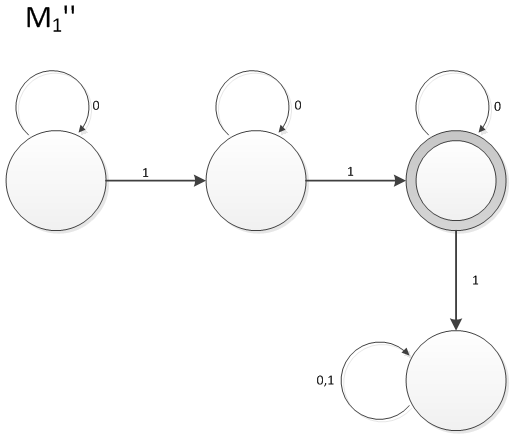
\includegraphics[scale=0.8]{figur2.png}
\caption{$M''_1$ er en DFA.}
\label{fig:2}
\end{figure}

\begin{figure}[h]
\centering
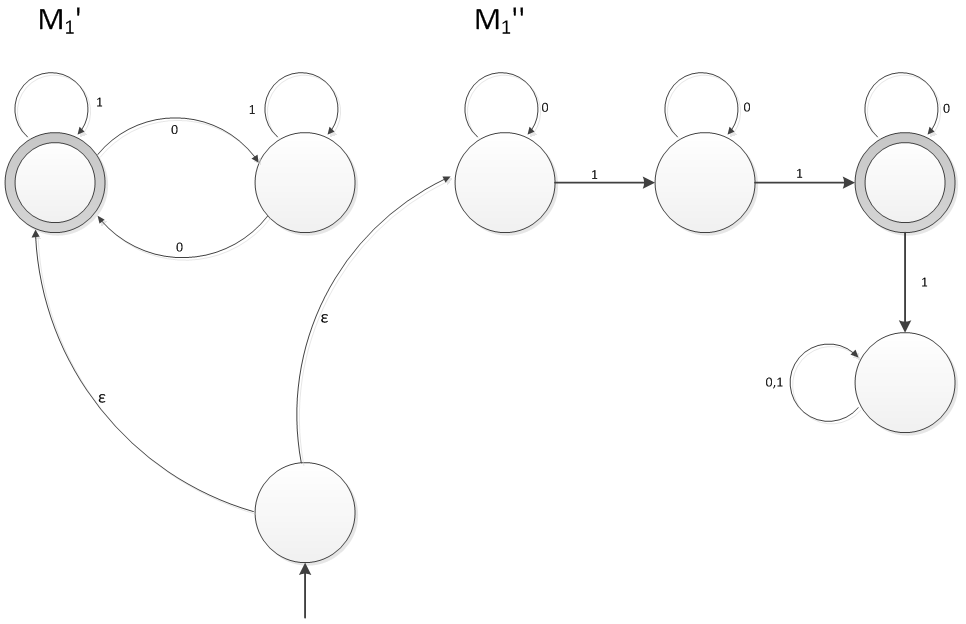
\includegraphics[scale=0.6]{figur3.png}
\caption{Dette er ikke en DFA -- men den kan genkende $L(M'_1) \cup L(M''_1)$.}
\label{fig:3}
\end{figure}

På Figur \ref{fig:1} og \ref{fig:2} kan ses de DFA'er der genkender $L_1'$ og $L_1''$.

Figur \ref{fig:3} viser tanken bag forsøget på at skabe en automat, der kan genkende $L'_1 \cup L''_2$. Den resulterende automat er ikke en DFA, for den har transitioner mærket med $\varepsilon$. 

Automaten er derimod en \emph{nondeterministisk endelig automat}. 

\begin{definition}
En NFA er en 5-tupel
%
\[ (Q,\Sigma,\delta,q_0,F)  \]
%
hvor
\begin{itemize}
\item $Q$  er en endelig mængde af tilstande
\item $\Sigma$ er alfabetet
\item $q_0$ er starttilstanden og $q_0 \in Q$
\item $\delta$ er overføringsfunktionen
\item $F$ er mængden af accepterede tilstande og $F \subseteq Q$
\end{itemize}

Lad $\Sigma_\varepsilon = \Sigma \cup \{\varepsilon\}$ så er
\[ \delta: Q \times \Sigma_\varepsilon \to \wp(Q) \]

\end{definition}

\chapter{NFA'er og DFA'er er ækvivalente}

\begin{eksempel}

Betragt sproget
%
\[L_2 = \{w \in \{a,b\}^{\ast} \mid w \text{ starter med $a$ eller starter med $ab$}\}\]
%
Dette sprog kan genkendes med NFA'en i Figur \ref{fig:4}. Bemærk at denne automatisk udviser nondeterminisme i og med at der fra nogle tilstande er mere end én transition med samme tegn og fra andre ikke nogen.

\begin{figure}[h]
\centering
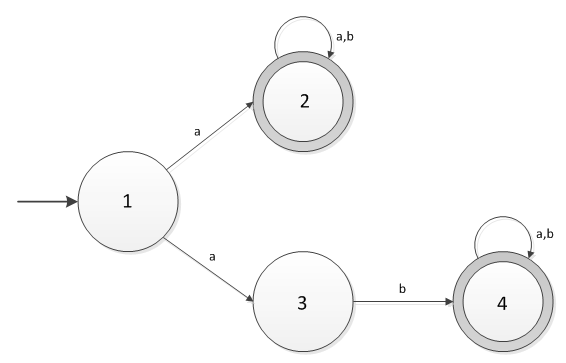
\includegraphics[scale=0.8]{figur4.png}
\caption{En NFA der genkender $L_2$.}
\label{fig:4}
\end{figure}

I denne automat har vi
%
\begin{align*}
Q & = \{1,2,3,4\} \\
\Sigma & = \{a,b\} \\
q_0 & = 1 \\
F & = \{2,4\} 
\end{align*}

$\delta$ er givet ved Tabel \ref{tab:1}.

\begin{table}[h]
\begin{center}
    \begin{tabular}{c|c|c|c|c|}
        ~ & 1     & 2   & 3   & 4   \\ \hline
        a & {2,3} & {2} & Ø   & {4} \\ \hline
        b & Ø     & {2} & {4} & {4} \\ \hline
        c & Ø     & Ø   & Ø   & Ø   \\
        \hline
    \end{tabular}
\end{center}
\label{tab:1}
\caption{Overføringsfunktionen for NFA i Figur \ref{fig:4}.}
\end{table}

\end{eksempel}

\begin{definition}
Lad $N = (Q,\Sigma,q_0,\delta,F)$ være en NFA. Lad $w \in a_1, ... , a_k \in \Sigma^{\ast}$
$w$ bliver accepteret af $N$ hvis $w = b_1 \ldots b_n$, hvor $b_i \in \Sigma_\varepsilon (1 \leq i \leq n)$, så $N$ ved at læse $b$'erne kan ende i en accepttilstand.

Dvs. der findes en følge af tilstande $r_0, ... , r_n$ så

\begin{itemize}
\item $r_0 = q_0$
\item $r_{i+1} \in \delta(r_i,b_i)$ for alle $0 \leq i < n$
\item $r_n \in F$
\end{itemize}

\end{definition}

\begin{eksempel}

\begin{figure}[h]
\centering
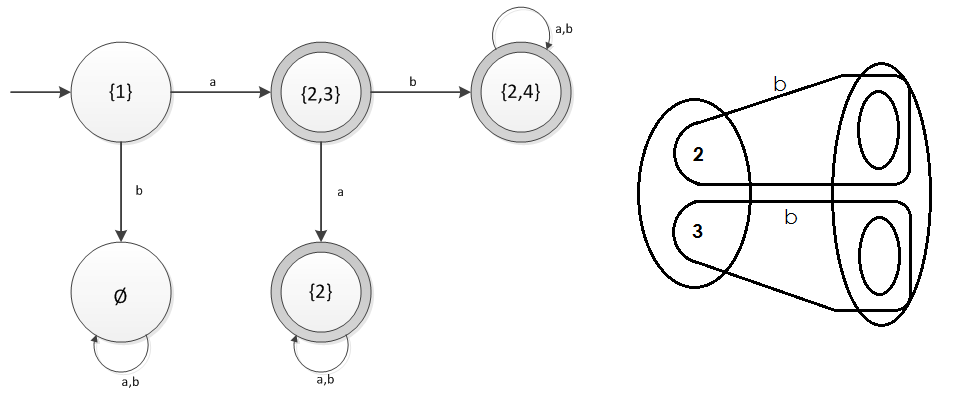
\includegraphics[scale=0.8]{figur6.png}
\caption{DFA lavet ud fra figur 4.}
\label{fig:6}
\end{figure}

På Figur \ref{fig:6} ses den DFA der er lavet ud fra Figur \ref{fig:4}. Princippet er at man fra den starttilstand man nu er i, ved et givent inçç
put ser hvad man kan nå til derfra med dette input. I dette eksempel undersøger man hvor man kan komme hen fra tilstand 2 og 3 med et input $b$.
\end{eksempel}

\begin{saetning}
For enhver NFA $N$ findes der en ækvivalent DFA $M$.
\end{saetning}

\begin{bevis}
Lad $N = (Q,\Sigma,q_0,\delta,F)$. Vi laver en DFA $M = (Q_1,\Sigma,q_1,\delta_1,F_1)$

Vi lader $Q_1 = \pow{Q}$, dvs. de nye tilstande i $Q_1$ er delmængder af de gamle tilstande fra $Q$. 

Først betragt en $N$ \emph{uden} $\varepsilon$-transitioner. I dette tilfælde har vi
%
\begin{align*}
q_1 & = \{q_0\} \\
F_1 & = \setof{R \in \pow{Q}}{ R \cap F \neq \emptyset} \\
\delta_1(R,x) & = \bigcup \limits_{r \in R}\delta(r,x)
\end{align*}
%
Accepttilstandene i den nye automat er således de mængder af gamle tilstande, som indeholder mindst én gammel accepttilstande. Dette skyldes at en streng ville blive accepteret af $N$ hvis der fandtes mindst én måde at læse strengen på således at automaten endte i en accepttilstand.

For en NFA med $\varepsilon$-transitioner indfører vi $\varepsilon$-aflukning.
Lad $R \in \wp(Q)$. Så definerer vi
%
\[E(r) = \setof{r \in Q}{ r \text{ kan nås fra en tilstand i $R$ med 0 eller flere $\varepsilon$-transitioner}}\] 
%
\begin{align*}
q_1 & = E(\{q_0\}) \\
\delta(R,x) & = E(\bigcup \limits_{r \in R}\delta(r,x))
\end{align*}
%
\end{bevis}

$\bigcup$ betyder her en \emph{itereret} foreningsmængde; sammenlign med sumtegnet $\sum_{1 \leq i \leq k} x_i$ der betegner summen $x_1 + \ldots + x_k$. 

\begin{eksempel}
\begin{figure}[h]
\centering
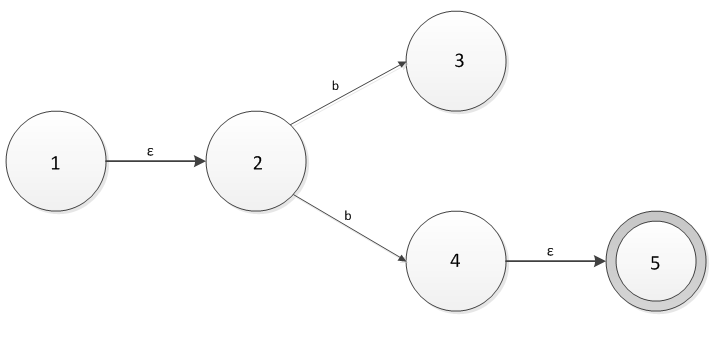
\includegraphics[scale=0.8]{figur7.png}
\caption{En NFA $N$}
\label{fig:7}
\end{figure}

\begin{figure}[h]
\centering
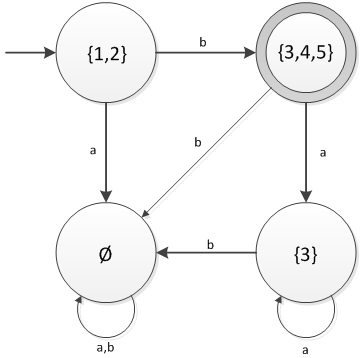
\includegraphics[scale=0.8]{figur8.png}
\caption{Den ækvivalente DFA $M$ (se Figur \ref{fig:7}).}
\label{fig:8}
\end{figure}

På Figur \ref{fig:7} kan ses NFA'en $N$. På Figur \ref{fig:8} kan ses den konstruerede DFA $M$ ud fra den oprindelige automat på Figur \ref{fig:7}.

Generelt kan vi risikere at der i den konstruerede DFA kan være $2^k$ tilstande, hvis der i den oprindelige NFA var $k$ tilstande.
\end{eksempel}

\chapter{De regulære sprog er lukket under $\cup$, $\circ$ og $\ast$.}

De \emph{regulære operationer} er defineret som
%
\begin{align*}
L_1 \cup L_2 &= \setof{x}{ x \in L_1 \lor x \in L_2} \\
L_1 \circ L_2 & = \setof{x}{ \exists u \in L_1, \exists v \in L_2, x = uv } \\
L^{\ast} & = \setof{x}{ x = w_1 \ldots w_k, k \geq 0, w_i \in L \text{ for } 1 \leq i \leq k}
\end{align*}
%
Vi kan nu vise at at de regulære sprog er lukket under de regulære operationer.

\begin{saetning}
Hvis $L_1$ og $L_2$ er regulære sprog, så er $L_1 \cup L_2$ regulært.
\end{saetning}
\begin{bevis}
Da $L_1$ og $L_2$ er regulære, findes der en NFA $N_1$ så $L(N_1) = L_1$ og en NFA $N_2$ så $L(N_2) = L_2$.

Lav en ny NFA $N_12$ så $L(N_12) = L(N_1) \cup L(N_2)$. $N_1$ kan ses på Figur \ref{fig:9}.


\begin{figure}[h]
\centering
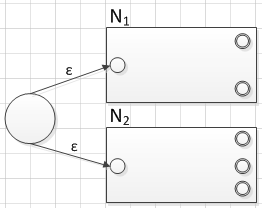
\includegraphics[scale=0.8]{figur9.png}
\caption{NFA der genkender $L(N_1) \cup L(N_2)$}
\label{fig:9}
\end{figure}

\end{bevis}

\begin{saetning}
Hvis $L_1$, $L_2$ er regulære sprog så er $L_1 \circ L_2$ regulært.
\end{saetning}

\begin{bevis}

Da $L_1$ er regulært, findes der en NFA $N_1$ så $L(N_1) = L_1$

Da $L_2$ er regulært, findes en NFA $N_2$ så $L(N_2) = L_2$

Vi laver en NFA $N_12$ så $L(N_12) = L_1 \circ L_2 = L(N_1) \circ L(N_2)$

\begin{figure}[h]
\centering
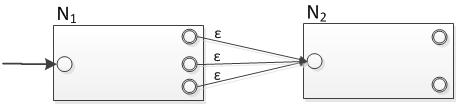
\includegraphics[scale=0.8]{figur10.png}
\caption{NFA der genkender $ L(N_1) \circ L(N_2)$}
\label{fig:10}
\end{figure}

Ideen er at forbinde $N_1$'s accepttilstande med $\varepsilon$-transitioner til $N_2$'s starttilstand -- \emph{kun} $N_2$'s accepttilstande skal forblive accepttilstande!

$N_1$ kan ses på Figur \ref{fig:10}.

\end{bevis}

\begin{saetning}
Hvis L er regulært, så er $L^{\ast}$ regulært.
\end{saetning}

\begin{bevis}
Da $L$ er regulært, er der en NFA $N$ så $L(N) = L$. Lav en NFA $N_1$ så $L(N_1) = L(N)^{\ast}$.

\begin{figure}[h]
\centering
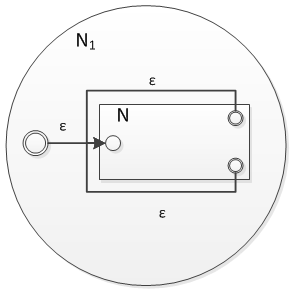
\includegraphics[scale=0.8]{figur11.png}
\caption{NFA der genkender $L(N)^{\ast}$.}
\label{fig:11}
\end{figure}

$N_1$ kan ses på Figur \ref{fig:11}.
\end{bevis}

\chapter{GYSER! - ``En finit kombination af et s{\ae}t af finale stadier''}

\section{Mange glemmer/misforstår $\varepsilon$-transitioner!}

Mange glemmer at man skal konstruere $\varepsilon$-aflukningen, når man konverterer en NFA til en DFA. Især glemmer mange, at den nye starttilstand er $\varepsilon$-aflukningen af den gamle.

\begin{figure}[h]
\centering
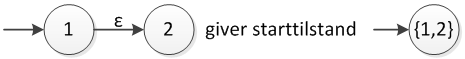
\includegraphics[scale=0.8]{figur12.png}
\caption{Den nye starttilstand er $\varepsilon$-aflukningen af starttilstanden i den oprindelige NFA.}
\label{fig:12}
\end{figure}

Et eksempel på dette kan ses på Figur \ref{fig:12}.

\section{``Alle kombinationer''}

En del studerende holder af at bruge pseudo-terminologi. ``Alle kombinationer'' er en tom upræcis betegnelse som nogle desværre bruger. Denne upræcise betegnelse kan blandt andet blive brugt om følgende udtryk.
%
\[ \pow{Q}, \Sigma^{\ast} \text{ og } A \times B \]
%
\emph{Lad være med det! Der er præcis terminologi!} Desuden hedder det ikke stadier men \emph{tilstande}! (Det engelske ord for ``stadie'' er \emph{stage}!)

\end{document}
